\documentclass[10pt,t]{beamer}

\usepackage[utf8]{inputenc}
\usepackage[T1]{fontenc}
\usepackage{graphicx}
\usepackage[caption=false]{subfig}
\usepackage{grffile}
\usepackage{longtable}
\usepackage{wrapfig}
\usepackage{rotating}
\usepackage[normalem]{ulem}
\usepackage{amsmath}
\usepackage{textcomp}
\usepackage{amssymb}
\usepackage{capt-of}
\usepackage{hyperref}

%\newcommand{\nitrous}{N$_2$O\xspace}
%\newcommand{\ozone}{O$_3$\xspace}

\input beamer_setup

\usetheme{default}
% ---------------------------------------------------------------------
% ---------------------------------------------------------------------
\begin{document}

\title[]{AIRS/CrIS Radiance Inter-Calibration: \newline
  Tests of Trends Using Time Series Combining Both Sensors}
\author{Chris Hepplewhite, Howard Motteler, Larrabee Strow}
\institute{Department of Physics, JCET\\
  University of Maryland Baltimore County (UMBC)}
\date{October 2, 2018}
% ---------------------------------------------------------------------
% ---------------------------------------------------------------------
\begin{frame}
  \titlepage
\end{frame}
% ---------------------------------------------------------------------
\begin{frame}
  \frametitle{Overview}
  \begin{itemize}
  \item A Hyperspectral IR Climate Record Depends on Sensor Continuity
  \item Spectral : Large differences between AIRS, CrIS, IASI
  \item Radiometric : Differences in the 0.3K or less range, which is a great starting point.
  \item Spatial : AIRS footprint slightly smeared relative to CrIS, slight impact on extrema.
    \item Sampling : different sensors sample the globe at slightly different times and atmospheric paths - requires stratergies such as equal area/equal weight.
    \item We explore here the differences between AIRS, SNPP CrIS, and NOAA20 CrIS.

  \end{itemize}
\end{frame}
% ------------------------------------------------------------------------------
\begin{frame}
  \frametitle{Some Spectral Considerations}

  \begin{itemize}
  \item Previous meetings and IEEE paper (publ. due) on AIRS2CrIS algorithm/product.
  \item Prerequisite for AIRS L1c at the DAAC for production of AIRS2CrIS products.
    \item Works well because AIRS SRFs are quite uniformly spaced, gaps filled and spectral overlap in wings of SRFs.
  \item Present approach: standardize on CrIS normal spectral resolution (NSR) for radiometric climate record.
  \item Conversion of IASI2CrIS is essentially trivial since IASI L1c gaussian apodization is far from zero at 0.8 cm path difference, so conversion to 0.8 sinc ILS is robust.
    \end{itemize}

\end{frame}
% -----------------------------------------------------------------------------
\begin{frame}
  \frametitle{Some Radiometric Considerations}
  \begin{itemize}
  \item Use a combination of SNOs and large statistical inter-comparisons to determine radiometric differences between sensors. They agree well. Although SNOs weighted to high latitudes, both methods permit scene dependencies to be analysed.
    \item Similar noise levels for AIRS2CrIS and CrIS if used for Level 2 retrievals.  To be incorporated into a AIRS2CrIS product.
  \end{itemize}
  
\end{frame}
% ----------------------------------------------------------------------------

\begin{frame}
  \frametitle{Example of One Month of AIRS:CrIS SNOs: Maps}
  \begin{center}
    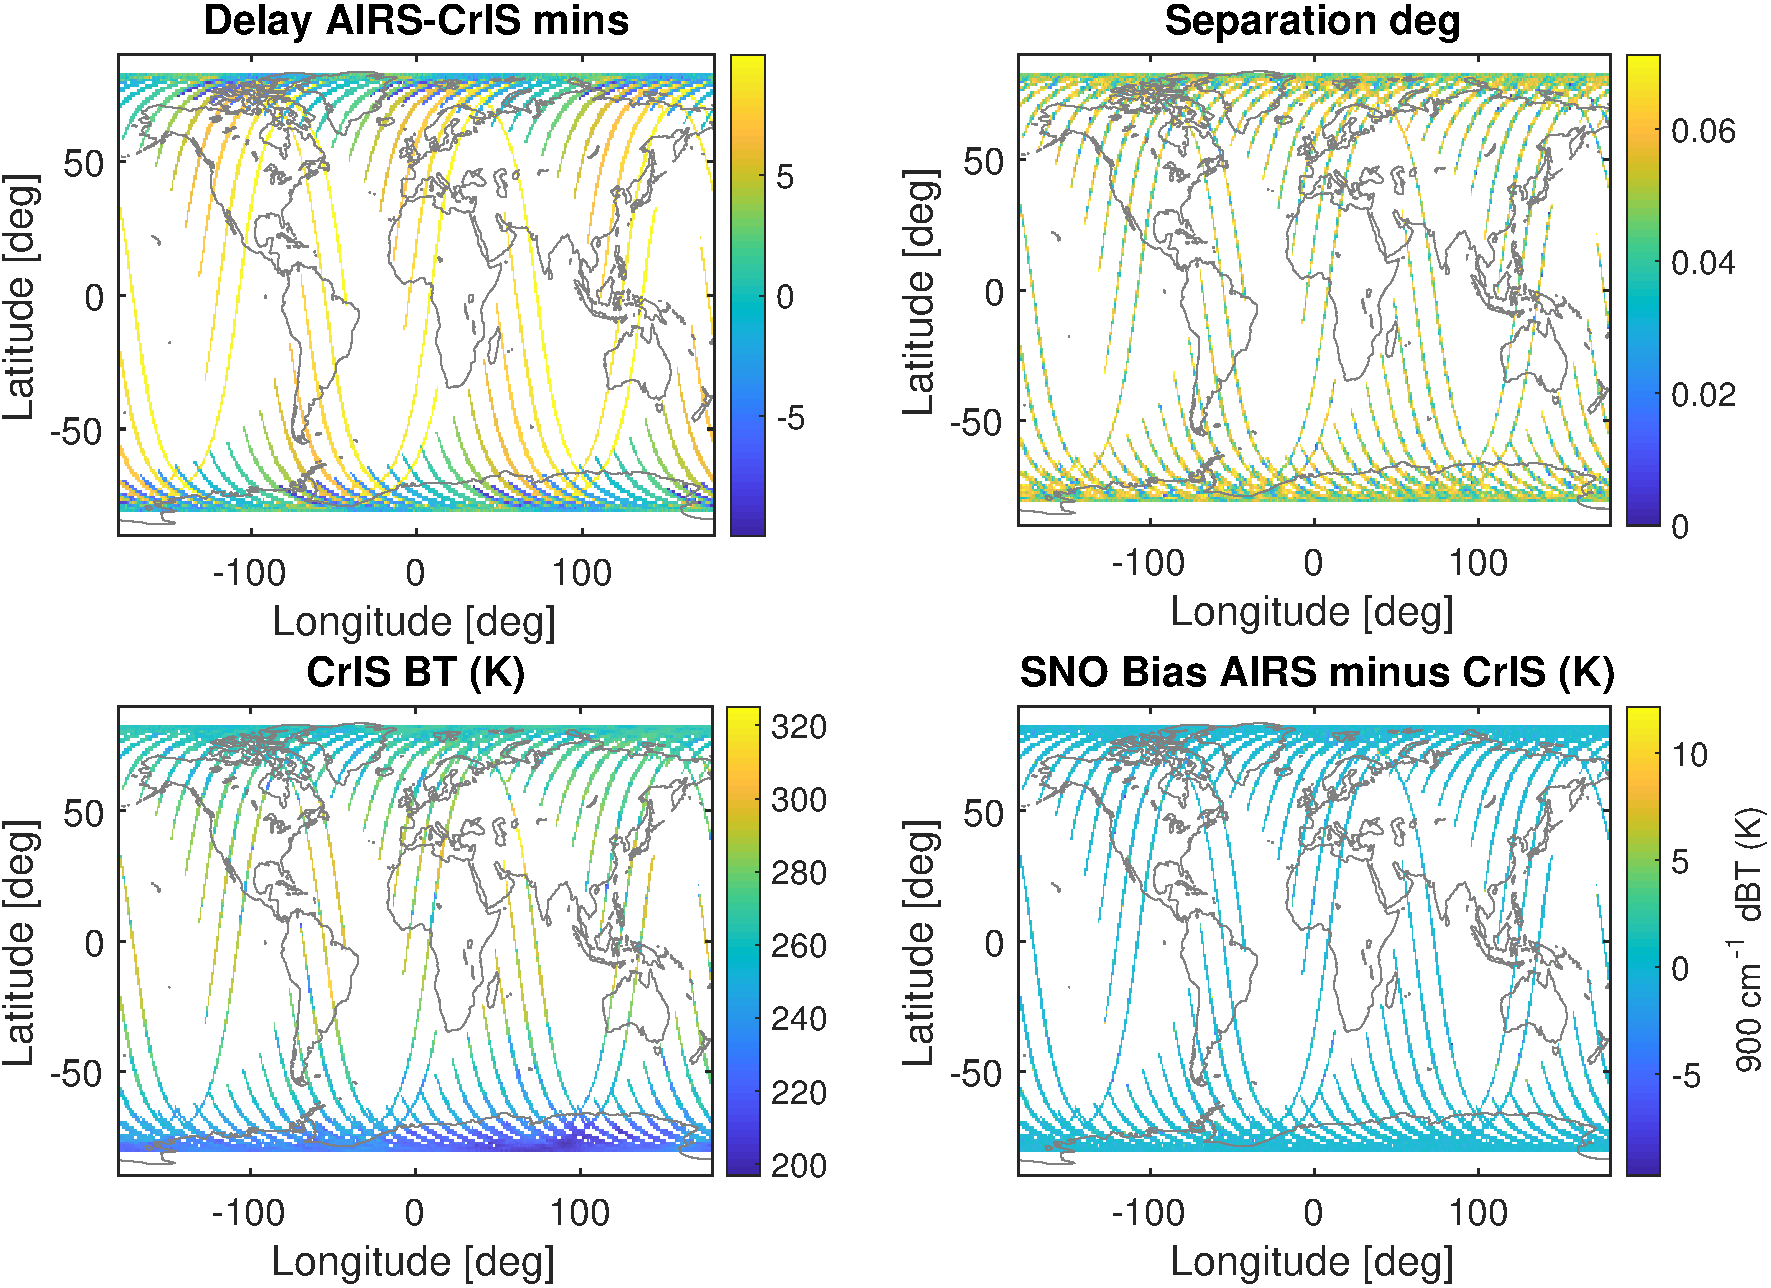
\includegraphics[width=0.95\linewidth]{./Figs/sno_ac1_lr_900wvn_aug2018_maps.pdf}
  \end{center}
  
\end{frame}
% --------------------------------------------------------------------
\begin{frame}
  \frametitle{Example of One Month of AIRS:CrIS SNOs: Bias}
  \begin{center}
    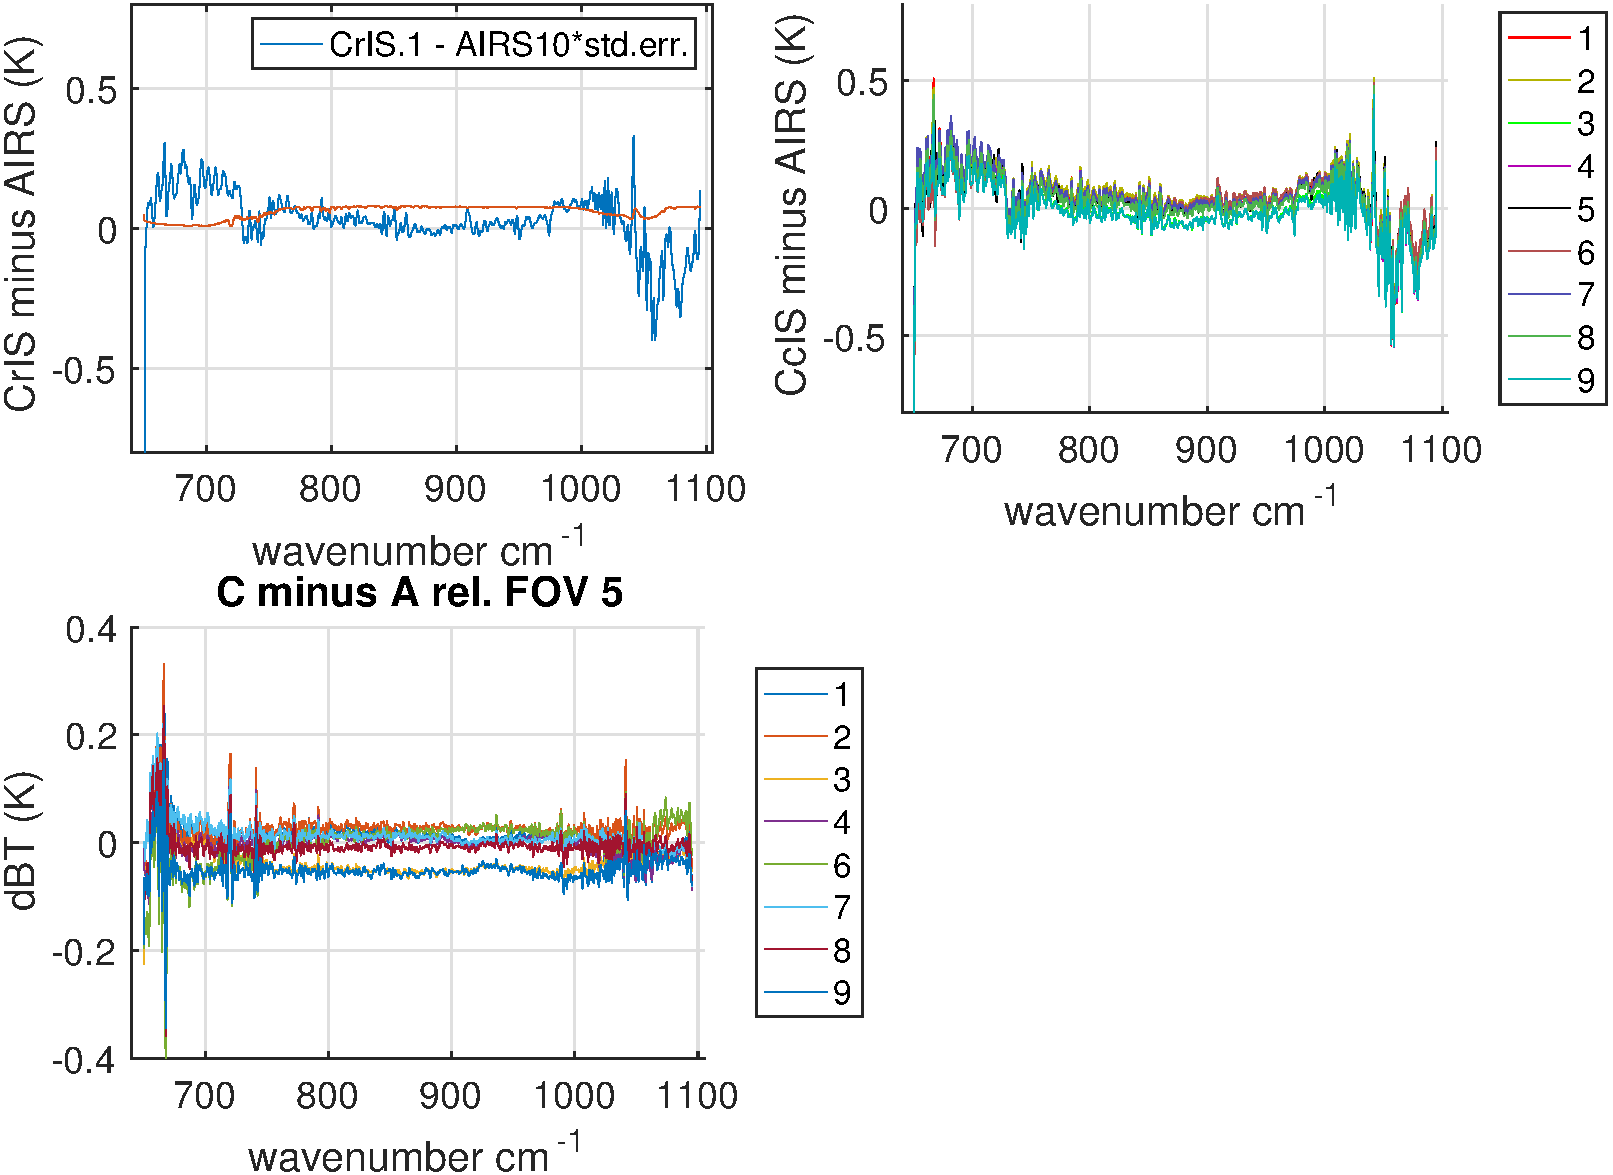
\includegraphics[width=0.95\linewidth]{./Figs/sno_ac1_lr_lw_mean_bias_jul2018.pdf}
  \end{center}
  
\end{frame}
% --------------------------------------------------------------------
\begin{frame}
  \frametitle{NPP vs N20 CrIS Using AIRS for Transfer}
  \begin{center}
    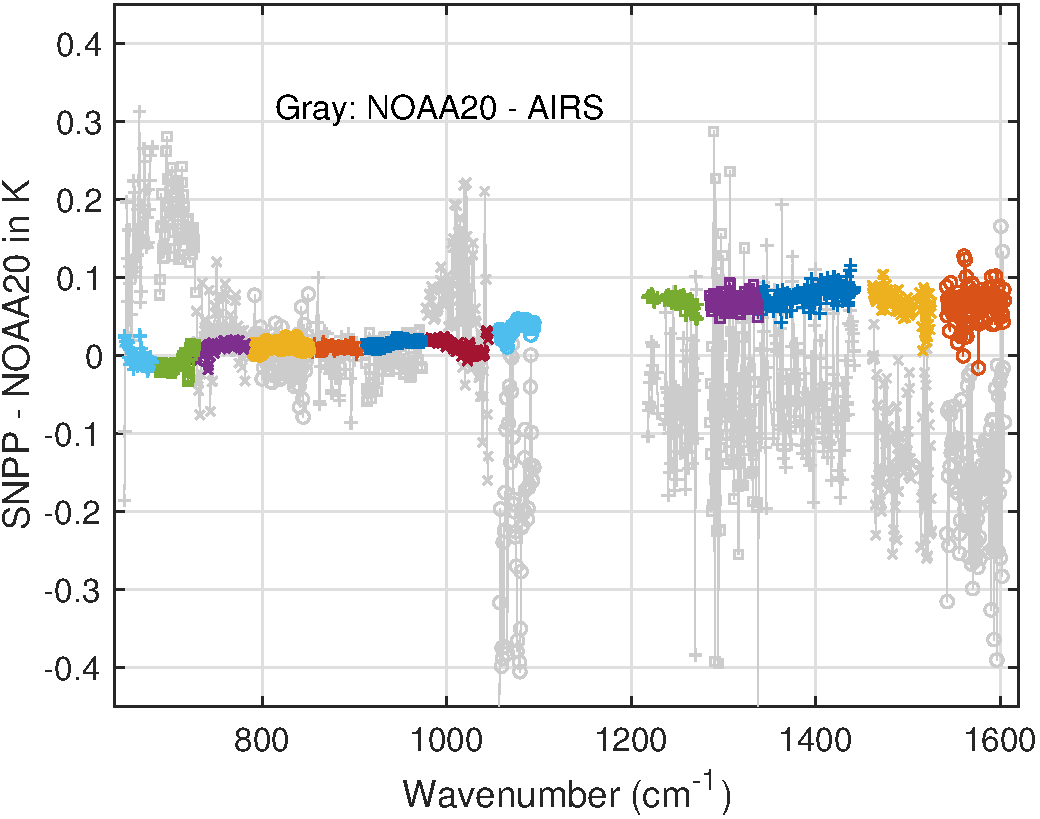
\includegraphics[width=0.75\linewidth]{./Figs/sno_march2018_snpp_minus_noaa20_with_c2_airs_ingrey.pdf}
  \end{center}
  \begin{itemize}
  \item AIRS is used as a cross-calibration transfer standard!
  \item NOAA-20 CrIS Calibration may be updated in the near future.
  \end{itemize}
  
\end{frame}
% --------------------------------------------------------------------
\begin{frame}
  \frametitle{Example Using AIRS SNOs to intercal NPP.CrIS and N20.CrIS }
  \begin{center}
    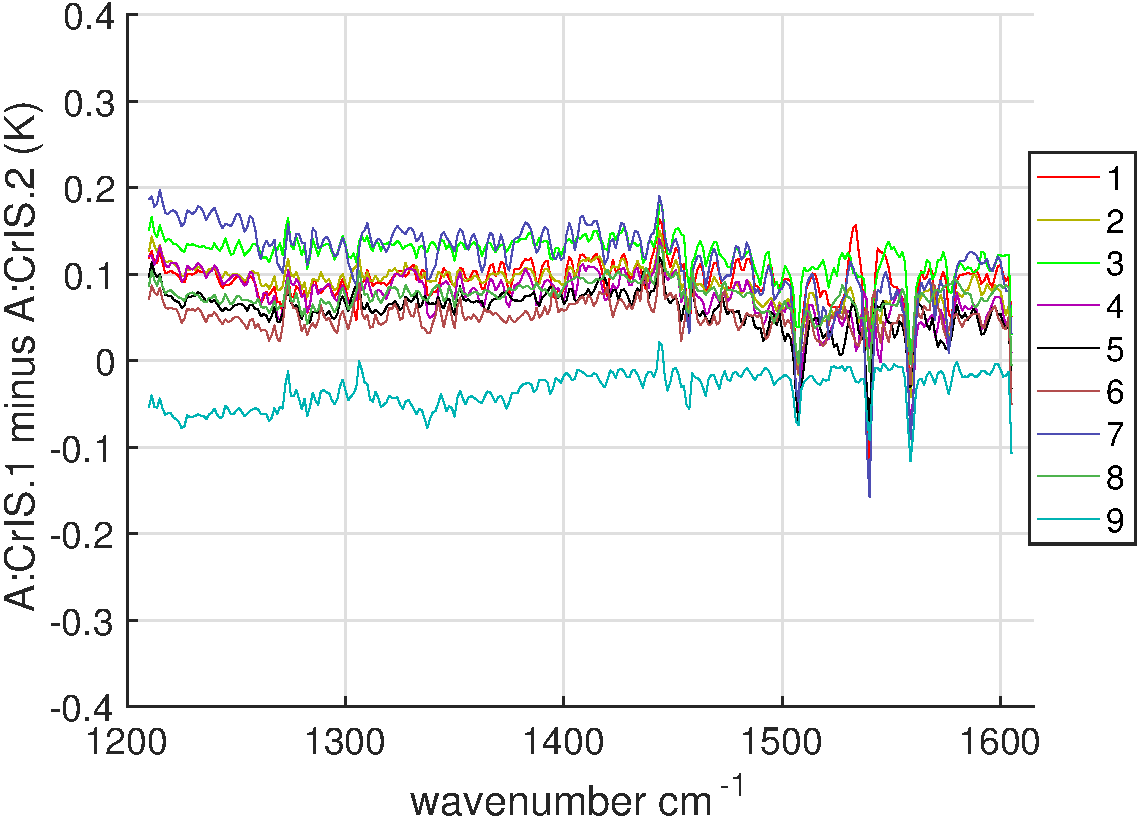
\includegraphics[width=0.95\linewidth]{./Figs/sno_ac1_ac2_dble_diff_lr_mw_cfov_2018febjun.pdf}
  \end{center}
  
\end{frame}
% --------------------------------------------------------------------
\begin{frame}
  \frametitle{Example Using IASI SNOs to intercal NPP.CrIS and N20.CrIS }
  \begin{center}
    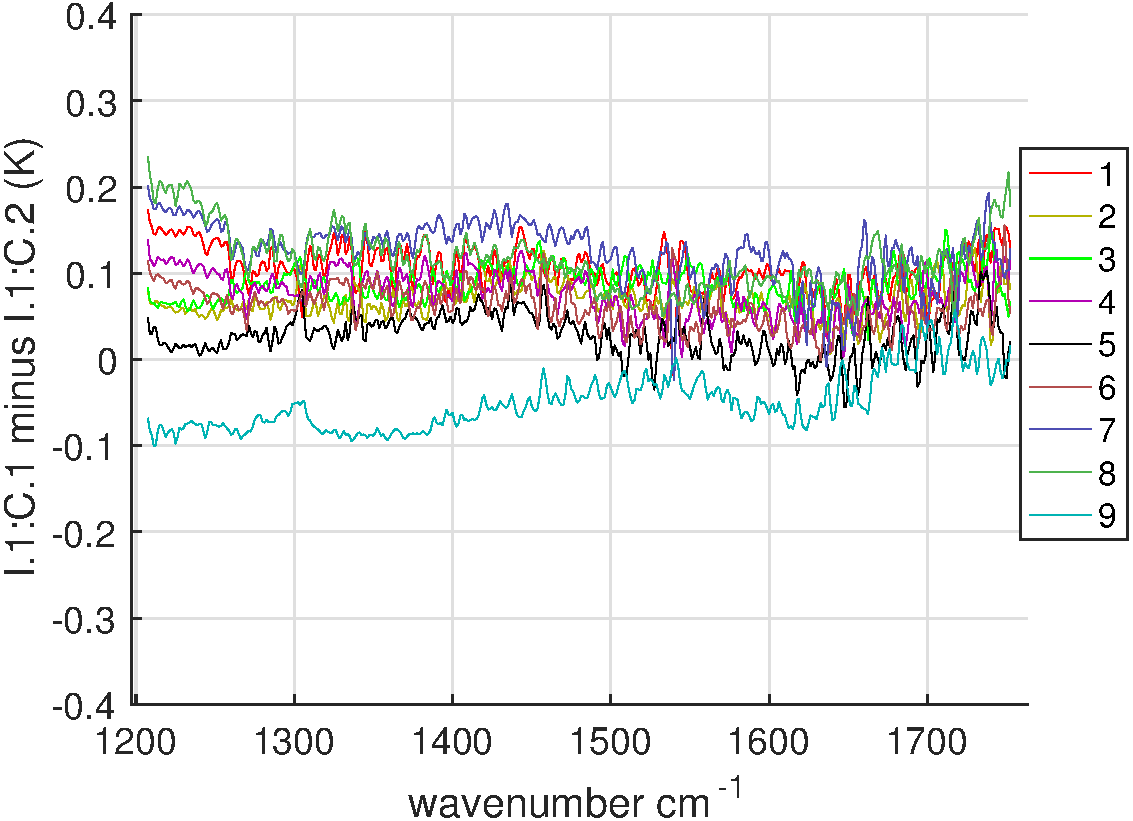
\includegraphics[width=0.95\linewidth]{./Figs/sno_i1c1_i1c2_dble_diff_lr_mw_2018febjun_aslp.pdf}
  \end{center}
  
\end{frame}
% --------------------------------------------------------------------
\begin{frame}
  \frametitle{How about MetOp-A/B IASI and NPP/N20 CrIS SNOs}
  \begin{center}
    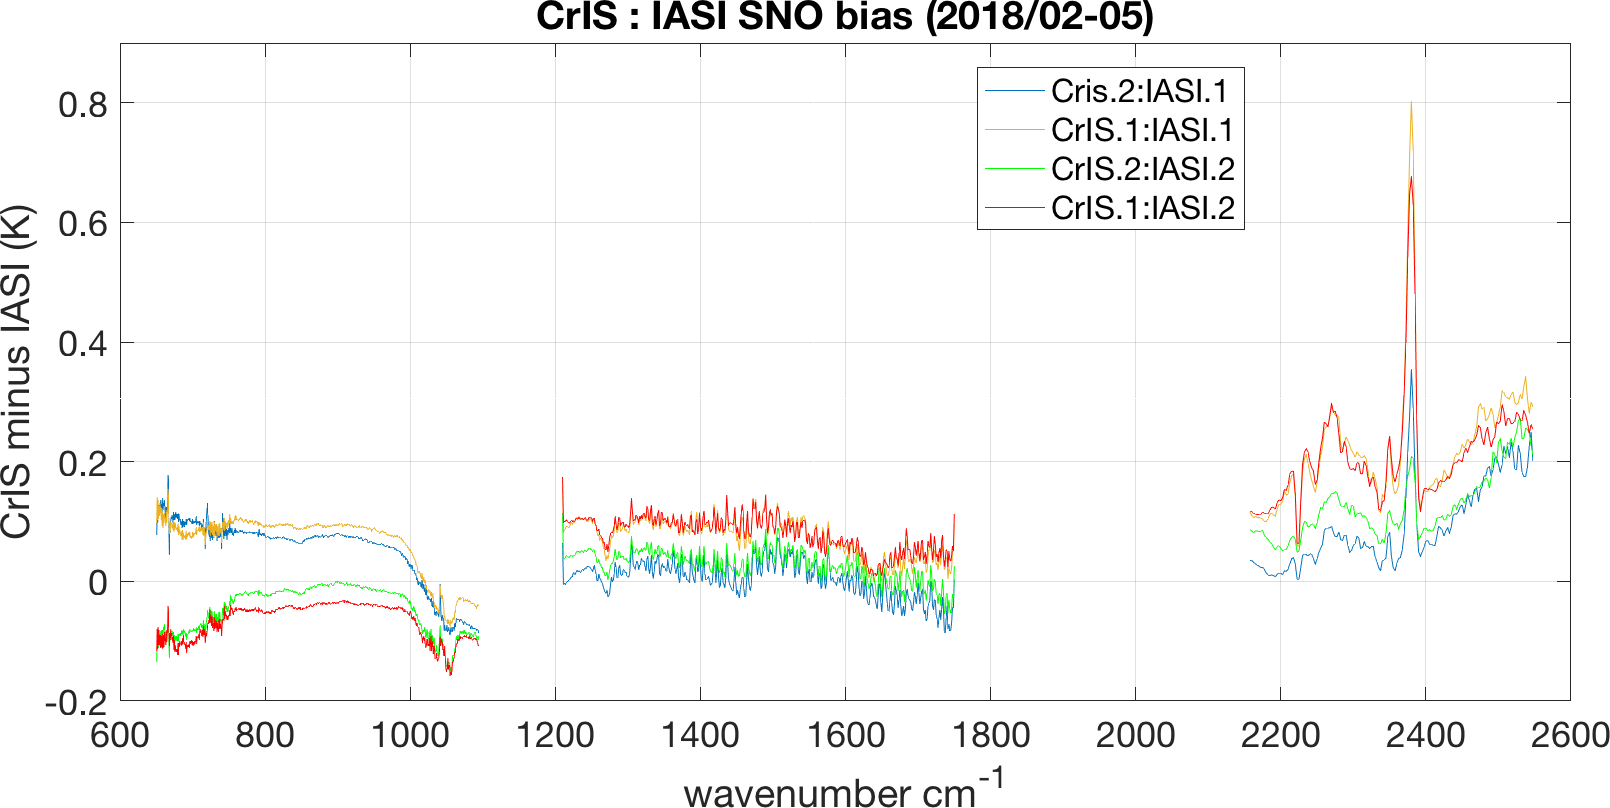
\includegraphics[width=0.95\linewidth]{./Figs/sno_iasi_cris_all_combin_mean_bias_spectral.png}
  \end{center}
  
\end{frame}
% --------------------------------------------------------------------
\begin{frame}
  \frametitle{AIRS:NPP.CrIS SNO and Random Stats Biases}
  \begin{figure}
    \centering
    \subfloat[2016 SNOs]{{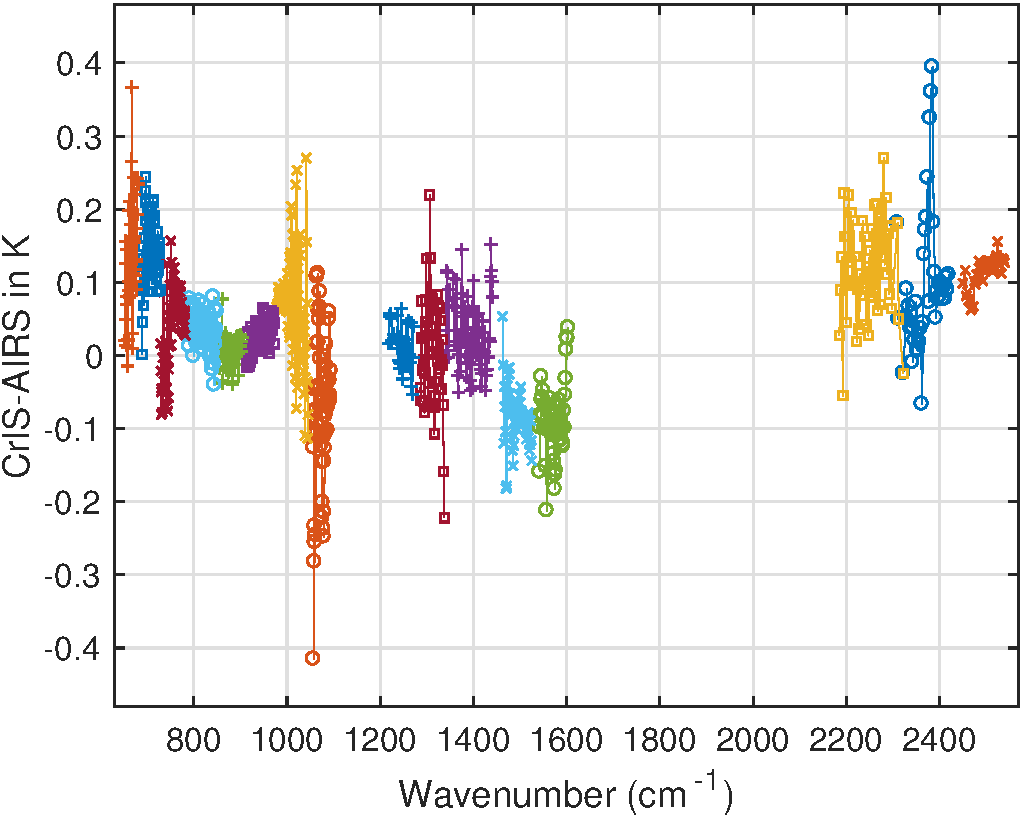
\includegraphics[width=5cm]{./Figs/snpp_vs_airs_sno.pdf} }}
    \qquad
    \subfloat[2016 Stats]{{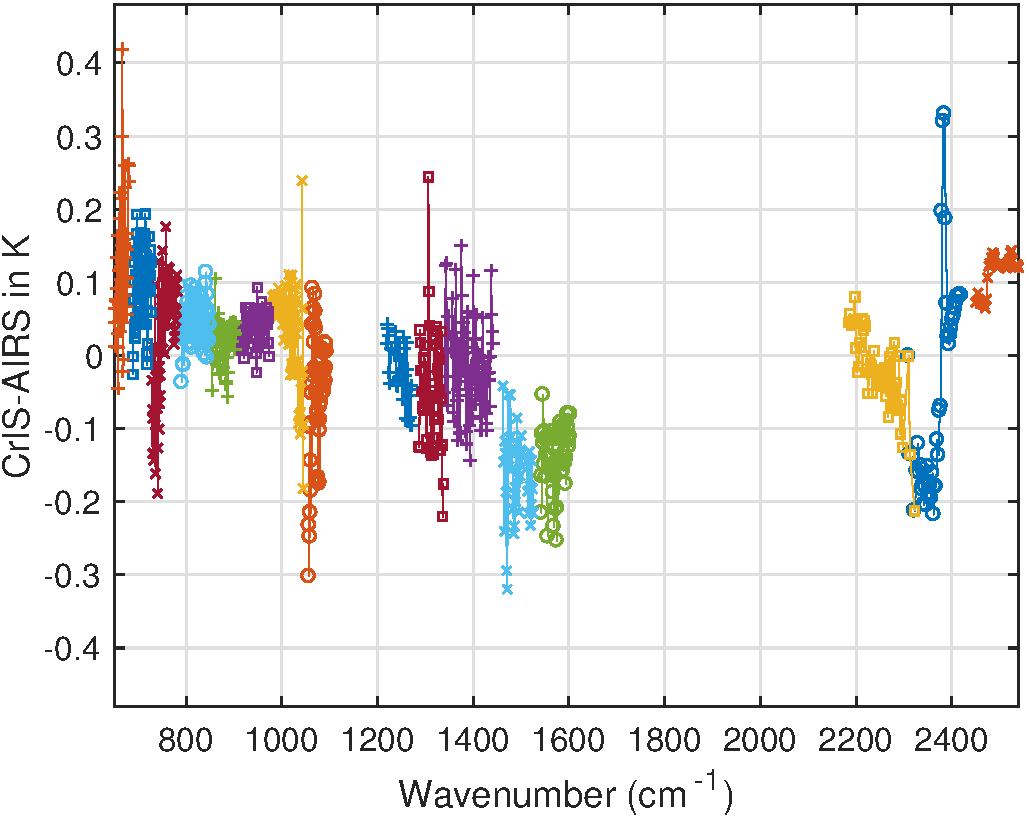
\includegraphics[width=5cm]{./Figs/snpp_vs_airs_stats.pdf} }}
  \end{figure}

  \small
  SNOs and random comparisons are in good agreement. Random averages are corrected to compensate for the larger mean secant viewing angle of CrIS vs AIRS and compared to SNOs.
\end{frame}
% --------------------------------------------------------------------
\begin{frame}
  \frametitle{Multi-year Mission Overlap Permits Bias Trending}
  \begin{figure}[]
    \subfloat[AIRS:CrIS 900wvn]{
      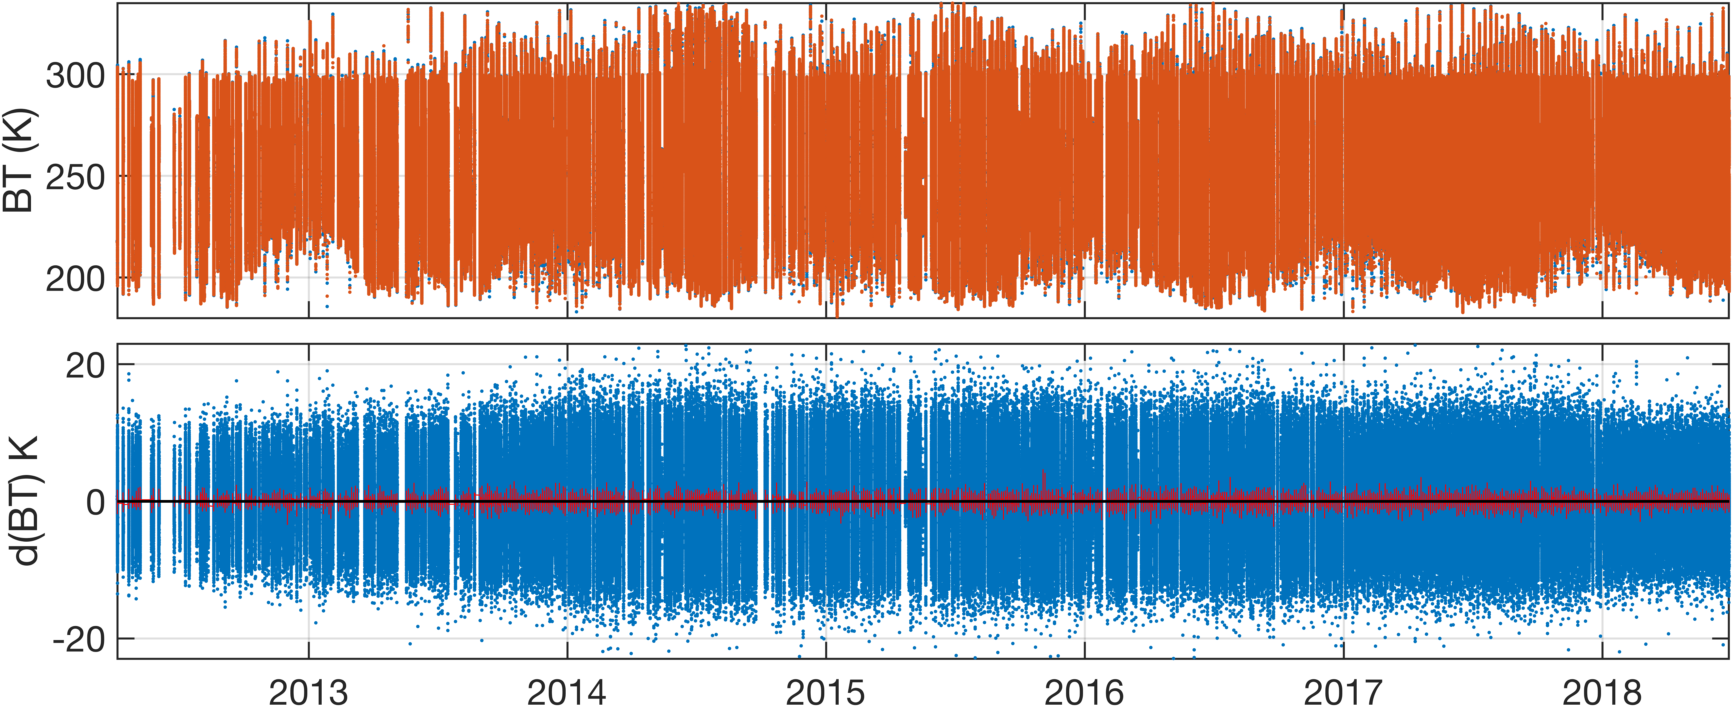
\includegraphics[width=0.66\linewidth]{./Figs/sno_ac1_lr_lw_window_trend_2012_18.png}}
    
    \subfloat[]{
      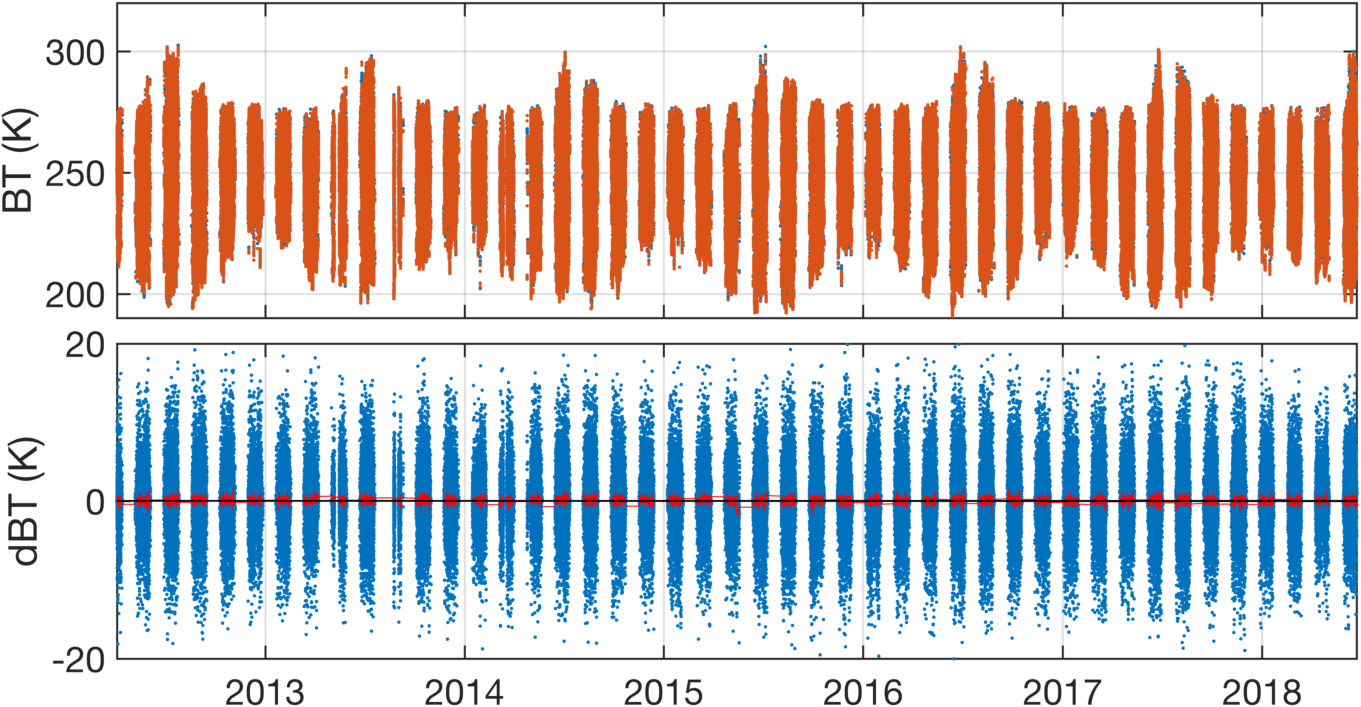
\includegraphics[width=0.66\linewidth]{./Figs/sno_i1c1_lr_lw_window_trend.png}}
    \end{figure}
    
\end{frame}
% --------------------------------------------------------------------
\begin{frame}
  \frametitle{}
  \begin{center}
  \end{center}
  
\end{frame}
% --------------------------------------------------------------------
\begin{frame}
  \frametitle{AIRS:CrIS Summary: LW Radiometric}
  \begin{itemize}
  \item Do AIRS SRF functions need adjustment:
    \item First, apply exact $\nu$ calibration to L1c (easy, just didn't do it)
      - ~8 $\wn$ "fringes" in CrIS-AIRS.  Entrance filter fringe shifts?
    \item Try ILS changes that are within estimated TVAC errors
    \item Then, apply as offsets in AIRS2CRIS
    \item \textcolor{maroon}{Testing does NOT require RTA calculations!}  AIRS ILS functions embedded in AIRS2CrIS algorithm.
      
  \end{itemize}
  
\end{frame}
% --------------------------------------------------------------------
\begin{frame}
  \frametitle{AIRS:CrIS SNO showing LW (mod 12) Variability}
  \begin{center}
    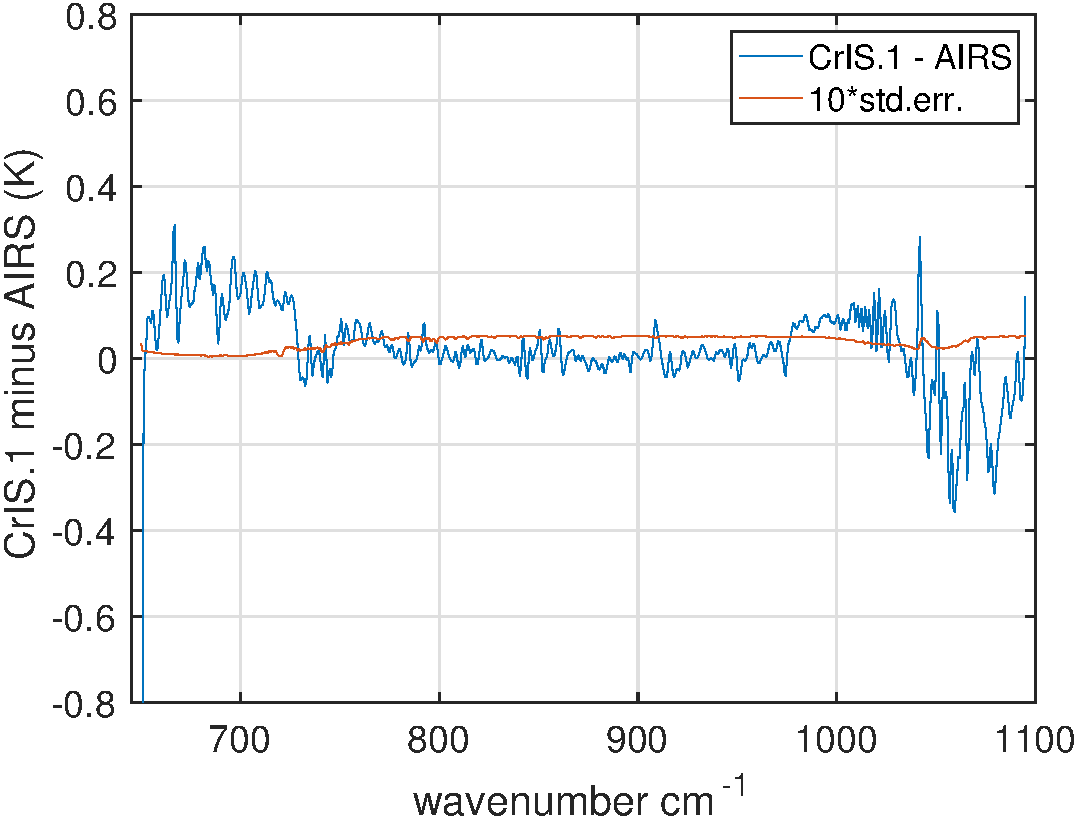
\includegraphics[width=0.95\linewidth]{./Figs/sno_ac1_lr_lw_2018d007e040_mean_bias.pdf}
  \end{center}
  
\end{frame}
% --------------------------------------------------------------------
\begin{frame}
  \frametitle{IASI:CrIS SNO showing LW detail}
  \begin{center}
    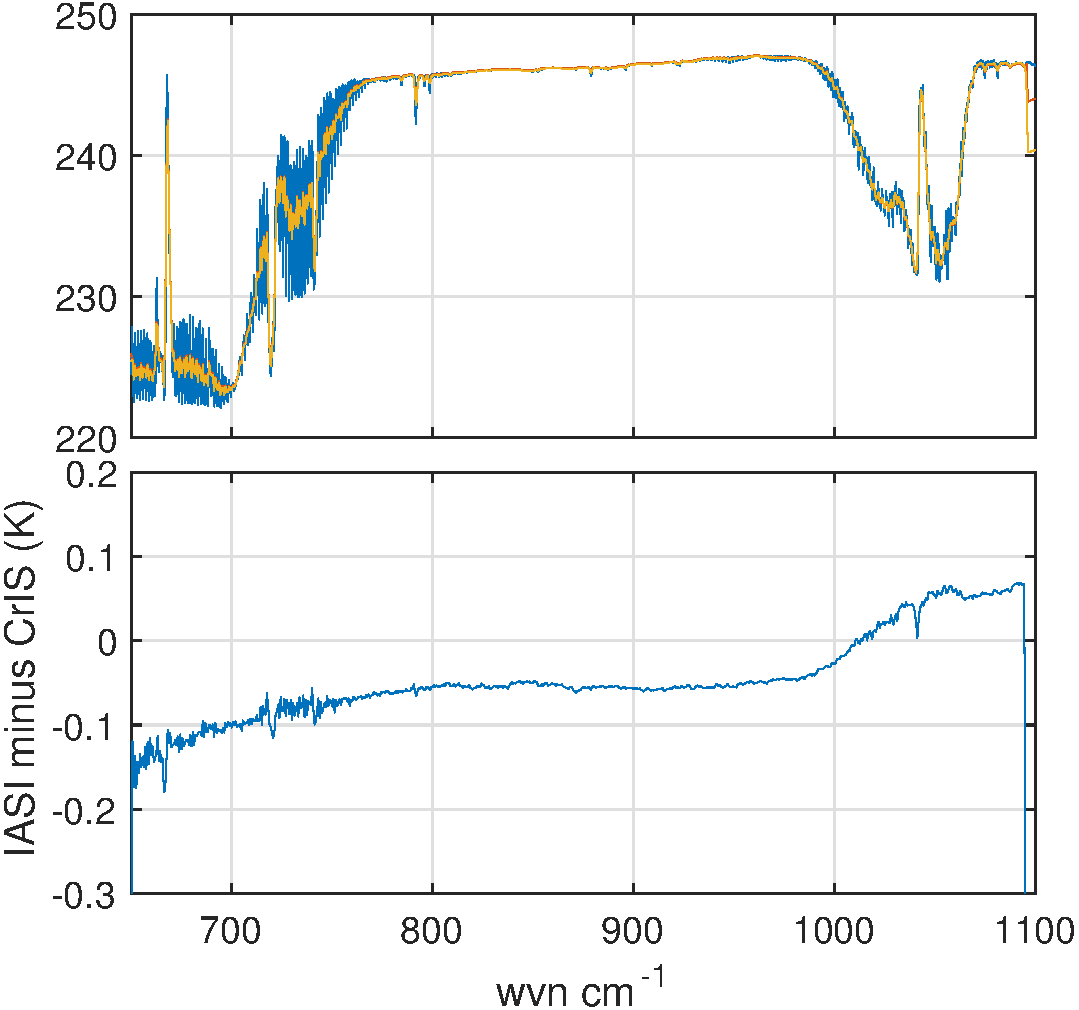
\includegraphics[width=0.8\linewidth]{./Figs/sno_i1c1_2018q1_lr_lw_mean_bias_null.pdf}
  \end{center}
  
\end{frame}
% --------------------------------------------------------------------
\begin{frame}
  \frametitle{Summary}
  \begin{itemize}
  \item We are looking at very small radiometric differences between all instruments.
  \item We use SNOs and large random (equal area weighted) statistical samples to inter-calibrate (radiometry).
  \item Instruments all appear very stable, so these differences can be account for.
  \item (If) we have enough overlap (true so far) the uncertainty in instrument differences is /very/ small, maybe <0.03K?
  \item Over 5-years that is <0.01K.
    
  \end{itemize}
  
\end{frame}
% --------------------------------------------------------------------

\end{document}
